\section*{Portable abstraction of hierarchical architectures for high-performance computing}





 \hypertarget{index_Introduction}{}\section{Introduction}\label{index_Introduction}
hwloc provides a portable abstraction (across OS, versions, architectures, ...) of the hierarchical topology of modern architectures. It primarily aims at helping high-performance computing applications with gathering information about the hardware so as to exploit it accordingly and efficiently.

hwloc provides a hierarchical view of the machine, NUMA memory nodes, sockets, shared caches, cores and simultaneous multithreading. It also gathers various attributes such as cache and memory information.

hwloc supports the following operating systems:

\begin{itemize}
\item Linux (including old kernels not having sysfs topology information, with knowledge of cpusets, offline cpus, and Kerrighed support) \item Solaris \item AIX \item Darwin \item OSF/1 (aka. Tru64) \item HP-UX \item Windows \item For other OSes, only the number of processors is available for now. \end{itemize}


For development and debugging purposes, hwloc also offers the ability to work on fake topologies:

\begin{itemize}
\item Symmetrical tree of resources generated from a list of level arities \item Remote machine simulation through the gathering of Linux sysfs topology files \end{itemize}


hwloc may also display the topology in a convenient format, either in graphical mode, or by exporting in PDF, PNG, FIG, ... format, or in text mode (see Examples below).

hwloc offers a programming interface for manipulating topologies and objects. It also brings a powerful cpu bitmap API that is used to describe topology objects location on physical/logical processors. See the \hyperlink{index_interface}{Programming interface} below. It may also be used to binding applications onto certain cores or memory nodes. Several utility programs are also provided to ease command-line manipulation of topology objects, binding of processes, ...

 \hypertarget{index_installation}{}\section{Installation}\label{index_installation}
hwloc (\href{http://www.open-mpi.org/projects/hwloc/}{\tt http://www.open-mpi.org/projects/hwloc/}) is available under the BSD license. It is hosted by Open MPI (\href{http://www.open-mpi.org/}{\tt http://www.open-mpi.org/}). The current SVN snapshot can be fetched with:

\begin{itemize}
\item svn checkout \href{http://svn.open-mpi.org/svn/hwloc/trunk}{\tt http://svn.open-mpi.org/svn/hwloc/trunk} hwloc-trunk \item cd hwloc-trunk \item ./autogen.sh \end{itemize}


Note that autoconf $>$=2.60, automake $>$=1.10 and libtool $>$=2.2.6 are required in that case.

Installation by itself is as usual:

\begin{itemize}
\item ./configure --prefix=... \item make \item make install \end{itemize}


Lstopo's fig support is always available. To get support for pdf, ps and png support, cairo is needed. To get support for xml, libxml2 is needed.

 \hypertarget{index_examples}{}\section{Examples}\label{index_examples}
On a 4-socket 2-core machine with hyperthreading, the {\tt lstopo} tool may show the following outputs:

 \begin{ImageNoCaption}\mbox{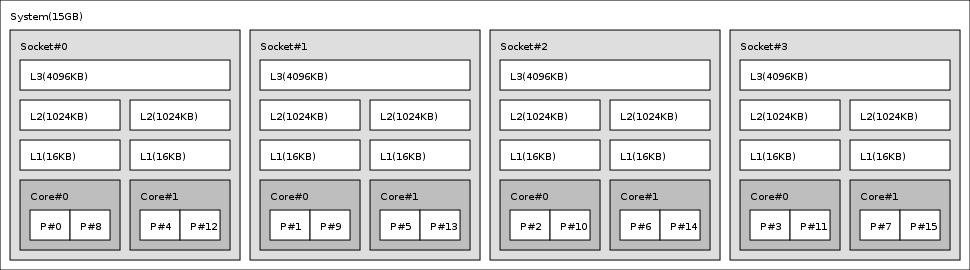
\includegraphics[width=\textwidth]{dudley.png}}
\end{ImageNoCaption}




\begin{Code}\begin{verbatim}System(15GB)
  Socket#0 + L3(4096KB)
    L2(1024KB) + L1(16KB) + Core#0
      P#0
      P#8
    L2(1024KB) + L1(16KB) + Core#1
      P#4
      P#12
  Socket#1 + L3(4096KB)
    L2(1024KB) + L1(16KB) + Core#0
      P#1
      P#9
    L2(1024KB) + L1(16KB) + Core#1
      P#5
      P#13
  Socket#2 + L3(4096KB)
    L2(1024KB) + L1(16KB) + Core#0
      P#2
      P#10
    L2(1024KB) + L1(16KB) + Core#1
      P#6
      P#14
  Socket#3 + L3(4096KB)
    L2(1024KB) + L1(16KB) + Core#0
      P#3
      P#11
    L2(1024KB) + L1(16KB) + Core#1
      P#7
      P#15
\end{verbatim}
\end{Code}



On a 4-socket 2-core Opteron NUMA machine, the {\tt lstopo} tool may show the following outputs:

 \begin{ImageNoCaption}\mbox{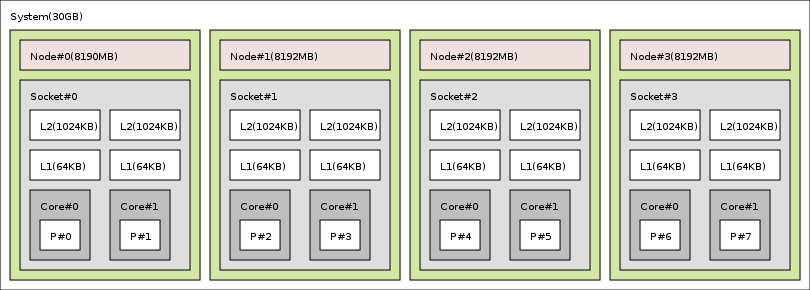
\includegraphics[width=\textwidth]{hagrid.png}}
\end{ImageNoCaption}




\begin{Code}\begin{verbatim}System(62GB)
  Node#0(8190MB) + Socket#0
    L2(1024KB) + L1(64KB) + Core#0 + P#0
    L2(1024KB) + L1(64KB) + Core#1 + P#1
  Node#1(8192MB) + Socket#1
    L2(1024KB) + L1(64KB) + Core#0 + P#2
    L2(1024KB) + L1(64KB) + Core#1 + P#3
  Node#2(8192MB) + Socket#2
    L2(1024KB) + L1(64KB) + Core#0 + P#4
    L2(1024KB) + L1(64KB) + Core#1 + P#5
  Node#3(8192MB) + Socket#3
    L2(1024KB) + L1(64KB) + Core#0 + P#6
    L2(1024KB) + L1(64KB) + Core#1 + P#7
  Node#4(8192MB) + Socket#4
    L2(1024KB) + L1(64KB) + Core#0 + P#8
    L2(1024KB) + L1(64KB) + Core#1 + P#9
  Node#5(8192MB) + Socket#5
    L2(1024KB) + L1(64KB) + Core#0 + P#10
    L2(1024KB) + L1(64KB) + Core#1 + P#11
  Node#6(8192MB) + Socket#6
    L2(1024KB) + L1(64KB) + Core#0 + P#12
    L2(1024KB) + L1(64KB) + Core#1 + P#13
  Node#7(8192MB) + Socket#7
    L2(1024KB) + L1(64KB) + Core#0 + P#14
    L2(1024KB) + L1(64KB) + Core#1 + P#15
\end{verbatim}
\end{Code}



On a 2-socket quad-core Xeon (pre-Nehalem ones assembling 2 dual-core dies into each socket):

 \begin{ImageNoCaption}\mbox{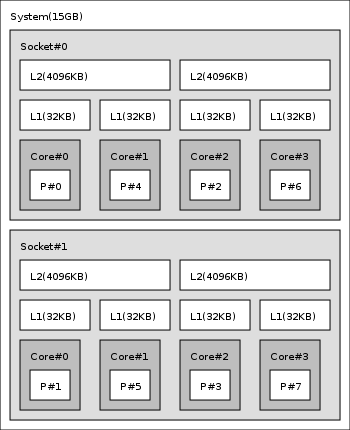
\includegraphics[width=\textwidth]{emmett.png}}
\end{ImageNoCaption}




\begin{Code}\begin{verbatim}System(15GB)
  Socket#0
    L2(4096KB)
      L1(32KB) + Core#0 + P#0
      L1(32KB) + Core#1 + P#4
    L2(4096KB)
      L1(32KB) + Core#2 + P#2
      L1(32KB) + Core#3 + P#6
  Socket#1
    L2(4096KB)
      L1(32KB) + Core#0 + P#1
      L1(32KB) + Core#1 + P#5
    L2(4096KB)
      L1(32KB) + Core#2 + P#3
      L1(32KB) + Core#3 + P#7
\end{verbatim}
\end{Code}



\hypertarget{index_interface}{}\section{Programming interface}\label{index_interface}
The basic interface is available in \hyperlink{hwloc_8h_source}{hwloc.h} . It mostly offers low-level routines for advanced programmers that want to manually manipulate objects and follow links between them. Most users should look at \hyperlink{helper_8h_source}{hwloc/helper.h} which provides a lot of interesting higher-level traversal examples.

Each object contains a cpuset which describes the list of processors that it contains. These cpusets may be used for \hyperlink{group__hwlocality__binding}{Binding}. hwloc offers an extensive cpuset manipulation interface in \hyperlink{cpuset_8h_source}{hwloc/cpuset.h} .

Moreover, hwloc also comes with additional helpers for interoperability with several commonly used environments. For Linux, some specific helpers are available in hwloc/linux.h , and \hyperlink{linux-libnuma_8h_source}{hwloc/linux-libnuma.h} if using libnuma. On glibc-based systems, additional helpers are available in \hyperlink{glibc-sched_8h_source}{hwloc/glibc-sched.h} . For systems with the Infiniband Verbs library, some dedicated helpers are provided in hwloc/ibverbs.h .

To precisely define the vocabulary used by hwloc, a \hyperlink{glossary}{Glossary} is available and should probably be read first.

Further documentation is available in html, manual pages, and pdf format in the source tarball in doc/doxygen-doc/ (after doxygen compilation for svn checkouts) and are installed in \$prefix/share/doc/hwloc/ and the usual manual repository.

The following section presents an example of API usage.\hypertarget{index_interface_example}{}\section{Interface example}\label{index_interface_example}
This section shows how to use hwloc with an small example {\tt hwloc-hello.c} that just prints the topology and binds itself to the first processor of the second core of the machine.

Hardware Location provides a pkg-config object, so compiling the example boils down to



\begin{footnotesize}\begin{verbatim}
CFLAGS+=$(pkg-config --cflags hwloc)
LDLIBS+=$(pkg-config --libs hwloc)
cc hwloc-hello.c $(CFLAGS) -o hwloc-hello $(LDLIBS)
\end{verbatim}
\end{footnotesize}




\begin{DocInclude}\begin{verbatim}/* topo-hello.c */
#include <hwloc.h>

static void print_children(hwloc_topology_t topology, hwloc_obj_t obj, int depth)
      
{
        char string[128];
        int i;

        hwloc_obj_snprintf(string, sizeof(string), topology, obj, "#", 0);
        printf("%*s%s\n", 2*depth, "", string);
        for (i = 0; i < obj->arity; i++)
                print_children(topology, obj->children[i], depth + 1);
}

int main(void)
{
        /* Topology object */
        hwloc_topology_t topology;

        /* Allocate and initialize topology object.  */
        hwloc_topology_init(&topology);

        /* ... Optionally, put detection configuration here to e.g. ignore some
           objects types, define a synthetic topology, etc....  The default is
           to detect all the objects of the machine that the caller is allowed
           to access.
           See Configure Topology Detection.  */

        /* Perform the topology detection.  */
        hwloc_topology_load(topology);


        /* Optionally, get some additional topology information
         * in case we need the topology depth later.
         */
        unsigned topodepth = hwloc_topology_get_depth(topology);


        /* Walk the topology with an array style, from level 0 (always the
         * system level) to the lowest level (always the proc level). */
        int depth, i;
        char string[128];
        for (depth = 0; depth < topodepth; depth++) {
                for (i = 0; i < hwloc_get_nbobjs_by_depth(topology, depth); i++) 
      {
                        hwloc_obj_snprintf(string, sizeof(string), topology,
                                        hwloc_get_obj_by_depth(topology, depth, i
      ), "#", 0);
                        printf("%s\n", string);
                }
        }

        /* Walk the topology with a tree style.  */
        print_children(topology, hwloc_get_system_obj(topology), 0);


        /* Print the number of sockets.  */
        depth = hwloc_get_type_depth(topology, HWLOC_OBJ_SOCKET);
        if (depth == HWLOC_TYPE_DEPTH_UNKNOWN)
                printf("The number of sockets is unknown\n");
        else
                printf("%u socket(s)\n", hwloc_get_nbobjs_by_depth(topology, dept
      h));


        /* Find out where cores are, or else smaller sets of CPUs if the OS
         * doesn't have the notion of core. */
        depth = hwloc_get_type_or_below_depth(topology, HWLOC_OBJ_CORE);

        /* Get last one.  */
        hwloc_obj_t obj = hwloc_get_obj_by_depth(topology, depth, 
      hwloc_get_nbobjs_by_depth(topology, depth) - 1);
        if (!obj)
                return 0;

        /* Get a copy of its cpuset that we may modify.  */
        hwloc_cpuset_t cpuset = hwloc_cpuset_dup(obj->cpuset);

        /* Get only one logical processor (in case the core is SMT/hyperthreaded)
      .  */
        hwloc_cpuset_singlify(cpuset);

        /* And try to bind ourself there.  */
        if (hwloc_set_cpubind(topology, cpuset, 0)) {
                char *str = NULL;
                hwloc_cpuset_asprintf(&str, obj->cpuset);
                printf("Couldn't bind to cpuset %s\n", str);
                free(str);
        }

        /* Free our cpuset copy */
        hwloc_cpuset_free(cpuset);

        /* Destroy topology object.  */
        hwloc_topology_destroy(topology);

        return 0;
}
\end{verbatim}
\end{DocInclude}


 \hypertarget{index_bugs}{}\section{Questions and bugs}\label{index_bugs}
Questions should be sent to the devel mailing list (\href{http://www.open-mpi.org/community/lists/hwloc.php}{\tt http://www.open-mpi.org/community/lists/hwloc.php}). Bug reports should be reported in the tracker (\href{https://svn.open-mpi.org/trac/hwloc/}{\tt https://svn.open-mpi.org/trac/hwloc/}).

 \hypertarget{index_history}{}\section{History / credits}\label{index_history}
hwloc is the evolution and merger of the libtopology (\href{http://runtime.bordeaux.inria.fr/libtopology/}{\tt http://runtime.bordeaux.inria.fr/libtopology/}) project and the Portable Linux Processor Affinity (PLPA) (\href{http://www.open-mpi.org/projects/plpa/}{\tt http://www.open-mpi.org/projects/plpa/}) project. Because of functional and ideological overlap, these two code bases and ideas were merged and released under the name \char`\"{}hwloc\char`\"{} as an Open MPI sub-project.

libtopology was initially developed by the INRIA Runtime Team-Project (\href{http://runtime.bordeaux.inria.fr/}{\tt http://runtime.bordeaux.inria.fr/}) (headed by Raymond Namyst (\href{http://dept-info.labri.fr/~namyst/}{\tt http://dept-info.labri.fr/$\sim$namyst/})). PLPA was initially developed by the Open MPI development team as a sub-project. Both are now deprecated in favor of hwloc, which is distributed as an Open MPI sub-project.

 
